\documentclass{article}
% I just added all the things, if you have problems build, try deleting the
% naggin packages, fat chance I don't even use it.
\usepackage{amsmath}
\usepackage{txfonts}
\usepackage{booktabs}
\usepackage{color}
\usepackage{bussproofs}
\usepackage{graphicx}
\usepackage{pifont}
\usepackage{qtree}
\usepackage{tikz}
\usepackage{amssymb}
\usetikzlibrary{automata,arrows,positioning,calc}
\usepackage{listings}
\usepackage{hyperref}
\newenvironment{scprooftree}[1]%
{\gdef\scalefactor{#1}\begin{center}\proofSkipAmount \leavevmode}%
{\scalebox{\scalefactor}{\DisplayProof}\proofSkipAmount \end{center} }

\newcommand{\brcell}[2][l]{%
	\begin{tabular}[#1]{@{}l@{}}#2\end{tabular}}

\begin{document}
\lstset{language=Java}
\author{Jappie Klooster}
\title{Agents and you, a brief summary}
\maketitle

\section{Introduction}
This will be an introduction to agents coming from someone who followed
` hbo informatica' as pre study.

In here I will write down the things I think are important.

\section{Modal logic}
% Before starting I just want to lay out the idea here, everytime I hear
% kripke, I imagine someone waving his arm and shouting KRIPKE in anger.
% Not that anyone will ever read these comments but its a funny idea.

This course was thought by John-Jules Meyer. The `theoretic' part focused
on the ideas behind the logics, while the `practical' focussed on writing
propper proofs. I guess I'll treat both in here.

There are 2 main sources of information I'll use, the slides by John Jules
and the modal logic paper for artificial intelligence by rosja mastop to help
me with the practical part. 
% In truth I didn't understand much of the practicals, just giving a bunch
% of examples is not a good way of teaching how to write proofs.
% This paper seems to explain it in a more structural way.

\subsection{Basic modal logic}
Express intensional (context/situation-sensitve) notations such as: 
Knowledge, Belief, Obligation, Action and Time.

\subsubsection{Modal langauge}

Imports all the things from propositional logic and is extended
with the modal operators ($\Box\phi,\Diamond\phi$) which can be read as:

\begin{tabular}{ll}
	Symbol & Definition \\ \toprule
	$\Box\phi$ & It is \emph{necesarry} that $\phi$ \\
	$\Diamond\phi$ & it is \emph{possible} that $\phi$

\end{tabular}

\noindent
Also $\neg\Box\neg\phi = \Diamond\phi$ and
$\neg\Diamond\neg\phi = \Box\phi$. So you could theoratically
drop one to create the other.
% where $\phi$ is an object I guess?

\paragraph{Semantics} Kripke %KRIPKE, *waves arm*.
model/frame $M=\langle S,\pi,R \rangle$

\begin{tabular}{ll}
	Symbol & Definition \\ \toprule
	% worlds implies mutability, states, well a state is by definition 
	% imutable. I'm pretty sure we want immutability in these kind 
	% off logics
	$S$ & Is a set of \emph{states (or worlds)} \\
	$\pi$ & Is a truth assignment function $\pi : S \times AT \to {tt, ff}$ \\
	$R$	& $R \subseteq S \times S$ is an \emph{accesibility relation}\\
\end{tabular}

\subsubsection{Interpertation}

\begin{center}
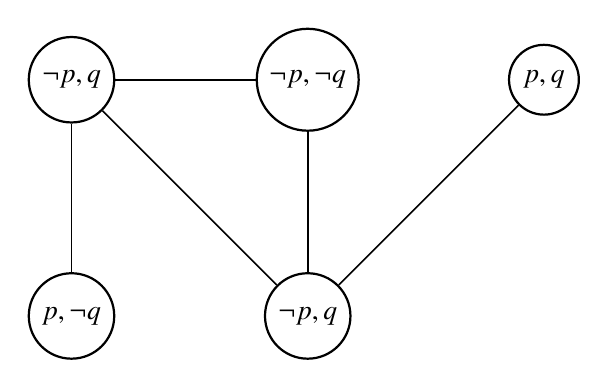
\begin{tikzpicture}[auto, >=stealth', auto, semithick, node distance=3cm]
\tikzstyle{every state}=[fill=white,draw=black,thick,text=black,scale=1]
\node[state]    (S)            {$\neg p, q$};
\node[state]    (A)[below of=S]{$p, \neg q$};
\node[state]    (B)[right of=S]{$\neg p, \neg q$};
\node[state]    (C)[right of=B]{$p, q$};
\node[state]    (E)[below of=B]{$\neg p, q$};
\path
(S)   edge[above]     		(A)
(S)   edge[above]     		(E)
(S)   edge[above]     		(B)
(B)    edge[above]     		(E)
(E)    edge[above]     		(C);
\end{tikzpicture}
\end{center}

Like classical propositional logic, but now realtive to a model and a state:

\[ M,s \vDash \phi \]

thus:

\begin{tabular}{lll}
	Modal & $\Leftrightarrow$ & Interpertation \\ \toprule
$M,s \vDash p$ & $\Leftrightarrow$ & $\pi(s,p) = tt$ \\
$M,s \vDash \phi \wedge \varphi $ & $\Leftrightarrow$ & $ M,s \vDash \phi
\mbox{ and }M,s\vDash \varphi$ \\
$M,s \vDash \Box \phi $ & $\Leftrightarrow$ & $ M,t \vDash \phi $ for 
\emph{every} $t$ such that $R(s,t)$ \\
$M,s \vDash \Diamond \phi $ & $\Leftrightarrow$ & $ M,t \vDash \phi $ for 
\emph{some} $t$ such that $R(s,t)$ \\\bottomrule
\end{tabular}

\subsubsection{Validity}
\begin{tabular}{llll}
	Definition & Denotation & $\Leftrightarrow$ & Interpertation \\ \toprule

$\phi$ is \emph{valid} in a model $M= \langle S, \pi, R \rangle$ &
$M\vDash\phi$ & $\Leftrightarrow$ & $M,s \vDash \phi$ for all $s \in S$ \\

$\phi$ is \emph{valid}  &
$\vDash\phi$ & $\Leftrightarrow$ & $M\vDash\phi$ for all Kripke models $M$ \\

$\phi$ is \emph{valid} wrt class $\zeta$ &
$\zeta\vDash\phi$ & $\Leftrightarrow$ & $M\vDash\phi$ for all Kripke models
$M \in \zeta$ \\\bottomrule
\end{tabular}

The last one doesn't occur often.

\subsection{System K}
We try to  axiomatize validities.

\paragraph{Axioms} We import all (or enough) propositional tautologies.
The K axiom ($(\Box\phi \wedge \Box (\phi \to \varphi))\to\Box\varphi$) is added.

\paragraph{Rules} Modes ponens
\begin{prooftree}
	\AxiomC{$\phi$}
	\AxiomC{$\phi \to \varphi$}
	\BinaryInfC{$\varphi$}
\end{prooftree}

Necisitation rule:
\begin{prooftree}
	\AxiomC{$\phi$}
	\UnaryInfC{$\Box\phi$}
\end{prooftree}

\subparagraph{Caution} the necisitation is different from the invalid
assertion: $\phi \to \Box \phi$.

\subsubsection{Derivability in K}
A \emph{derivation} of a formula $\phi$ is a finite sequence of formulas
$\phi_1, \dots \phi_n = \phi$. where each $\phi_i$ for $1 \ge i \ge n$
is either an instance of the acioms (or rather axiom schemes), or the
conclusion of one of the rules of which the premises have
been derived already, i.e{.} appear as $\phi_j$ in the sequance with
$j < i$.

% sad thing is I understand this crap now.
When we can derive an epistemic formula $\phi$ by using the axioms
and rules of $K_{(m)}$ we write $K_{(m)} \vdash \phi$

System $K_{(m)}$ is \emph{sound and complete}. This means
that exactly ll valid modal assertions can be obtained by derivations in
system $K_{(m)}$.

\[\vDash \phi \Leftrightarrow K_{(m)} \vdash \phi\]

% I leave out the (non) theoroms, it seems overkill.

\subsection{Dynamic logic}
An example of an (indexed) version of system $K$ is dynamic logic,
wehre the $\Box$ modality is associated with the execution results of
a program / action.

$\Box_\alpha$, normally written $[\alpha]$ 
with reading $[\alpha]\phi$: after exuction of $\alpha$ it holds that $\phi$

\[<\alpha>\phi = \neg [\alpha] \neg \phi \]

\subsubsection{Semantics}
Accessibility relation $R_\alpha$ for every action $\alpha$

\begin{tabular}{llll}
	% I added the natural collumn, because otherwise I won't remember.
	% Translating something in a different notation is stupid.
	notation & = & definition & natural \\ \toprule
	$R_{\alpha;\beta}$ & = & $R_\alpha \circ R_\beta$ &
	execute from $R_\alpha$ until including $R_\beta$\\
	$R_{\alpha+\beta}$ & = & $R_\alpha \cup R_\beta$ &
	execute $R_\alpha$ or $R_\beta$\\
	$R_{\alpha*}$ & = & $R_\alpha*$ &
	Execute an arbitrary times \\ \bottomrule
\end{tabular}

\subsubsection{Interpertation}
\begin{tabular}{lll}
	Modal & $\Leftrightarrow$ & Interpertation \\ \toprule
	$M,s \vDash [\alpha]\phi$ & $\Leftrightarrow$ &
	for all $s'$ with $R_\alpha(s,s'): M,s' \vDash \phi$ \\
	$M,s \vDash <\alpha>\phi$ & $\Leftrightarrow$ &
	for some $s'$ with $R_\alpha(s,s'): M,s' \vDash \phi$ \\\bottomrule
\end{tabular}

\subsection{Special properties of accessibility relations}
\begin{tabular}{lll}
	R is \dots& if\dots & natural language \\ \toprule
	reflexive & $\forall s \in S(s,s) \in R$ & all s are linked with 
	themselves\\

	transitive & $\forall s,t,u \in S:(s,t) \in R \& (t,u) \in R \Rightarrow
	(s,u) \in R$ & \brcell{if s is related to t, and t is related to u,  \\
		then s has a relation with u, \\ in other words, you can make shortcuts}\\

	symmetrical &$\forall s,t \in S:(s,t) \in R \Rightarrow (t,s) \in R$ &
	undirected, can go back and forth\\
	euclidiean & $\forall s,t,u \in S:(s,t) \in R \& (s,u) \in R \Rightarrow
	(t,u) \in R$ & \brcell{if s has a relation with t and u, then u and t \\
	have a relation to, you can make triangles.} \\
	serial & $\forall s \in S \exists t \in S (s,t) \in R$&
	\brcell{All states in S are connected to \\ at least one other state in S}\\
	an equivalance relation& R is \emph{reflexive, transitive and 
	symetrical}& \brcell{the states R links to have something in \\ 
	common (not equal?)} \\ \bottomrule
\end{tabular}
\section{APL}
Medhi dastani taught about the agent programming langauge (APL).
\subsection{Agent data structure}
This represents the mental state of a agent. \\
\begin{tabular}{ll}
	Name & Does what \\ \toprule
	Beliefs & Information available to the agent \\
	Goals & Objectives that the agent wants to achieve \\
	Events & Obsevations of (environmental) changes \\
	Capabilities & Actions that the agent can perform \\
	Plans & Procedures to achieve objectives \\
	Reasoning rules & Reason about goal and plans \\
\end{tabular} \\

\noindent
The rules can be:

\begin{itemize}
	\item Planning rules (goal $\to$ plan)
	\item Procedural rules (events $\to$ plan)
	\item Plan repair rules (plan $\to$ plan)
\end{itemize}

\subsection{Processing mental states}

\begin{itemize}
	\item Generate plans for received events.
	\item Generate plans for goals.
	\item Process exceptions and handle failures.
	\item Repair plans.
	\item Select plans for execution.
	\item Execute plans.
\end{itemize}

\subsection{Operational semantics}
Operational semantics defines the computation steps a program
configuration may take. Operational semantics allows studying
of programming constructs in a rigorous manner. It facilitates proving
general properties about a language. It lies close to the implementation
of an interpreter. It facilitates model checking.

\subsubsection{Basic syntax}
The configuration $C$ evolves into configuration $C'$:

\[C \to C'\]

If premise $P$ holds transition $C \to C'$ can be derived:

\begin{prooftree}
	\AxiomC{$P$}
	\UnaryInfC{$C \to C'$}
\end{prooftree}

\subsection{Configuration}
configurations only mention things that change.
Multi-agent configuration where $A$ is an agent and $\chi$ is the
environment:

\[\langle \{A_1, \cdots, A_n\}, \chi\rangle \]

Individual agent configuration where $i$ is the agent number, $\sigma$ the
believes, $\gamma$ the goals, $\Pi$ the plans $\theta$ the assignments and
$\xi$ the events:

\[A_i = \langle i, \sigma_i, \gamma_i, \Pi_i, \theta_i, \xi_i \rangle \]

\subsection{Transitions}
The confiugrations described \emph{what} can change where transition
will describe \emph{how} they can change.

$\vDash$ Describes a first order entailment relation. As I understand
this means $A \vDash B$ there exsits a $B$ in $A$ which has an entailment
to $A$. So $A$ is a set of things and a $B$ like thing exists in $A$.
\subsubsection{Belief update}
Execution of a belief update action $\alpha$ modifies the belief and goal
bases. $Update$ is an update function that is specified by the believe
update actions and $\gamma'=\gamma - \{\psi \in \gamma | \sigma' \vDash \psi\}$.
Which basically says that $\gamma'$ is equal to $\gamma$ minus the update.

\begin{prooftree}
	\AxiomC{$Update(\sigma, \alpha\theta)=\sigma'$}
	\UnaryInfC{$\langle i, \sigma, \gamma, \{(\alpha,id)\}, \theta, 
		\xi\rangle \to 
	\langle \langle i, \sigma', \gamma', \{\}, \theta, \xi\rangle$}

\end{prooftree}

So on the left side of the arrow, the plan is to do a believeUpdate $\alpha$
on the right side this is done so its removed from the plans and the believes
\emph{and} goals are modified. The goals are modified to because if a believe
with the same name as a goal becomes true than the goal is removed. (this is
a design decision btw, its just how 2apl works).

\subsubsection{Adopta goal}
Execution of a goal adopt action adopta(g) adds the goal to the beginning of
the goal base. If the goal $g$ trough assignment $\theta$ does not already
exists in goalbase.

\begin{prooftree}
	\AxiomC{$\sigma \nvDash g\theta$}
	\UnaryInfC{$\langle 
		i, \sigma, [\gamma_1, \cdots, y_n], \{(adopta(g),id)\}, \theta, \xi, 
	\rangle \to \langle 
		i, \sigma, [g\theta,\gamma_1, \cdots, y_n], \{\}, \theta, \xi, 
	\rangle$}
\end{prooftree}

So the agent comes accross a adopta method in the plan base $\Pi$, if
the associated believe of the goal is not true then you can start adding
it.
\subsubsection{Applying planning goal rules}
The structure of a PG-rule in 2apl is as follows:

\[\kappa <- \beta | \pi \]

Where $\kappa$ is the name of the plan.
$\beta$ is the condition that is applied before
executing the plan (basically a big if around the plan). $\pi$ is
the body of the plan, a set of instructions.

\begin{prooftree}
	\AxiomC{$\gamma \vDash \kappa \tau_1 \quad \& \quad
	\sigma \vDash \beta \tau_1 \tau_2$}
	\UnaryInfC{$\langle
		i, \sigma, \gamma, \Pi, \theta, \xi
	\rangle \to \langle
	i, \sigma, \gamma, \Pi \cup \{ \pi \tau_1 \tau_2 \}, \theta, \xi
	\rangle$}
\end{prooftree}

The transition can be executed if $\kappa$ is an active goal (this valuation
is stored in $\tau_1$ \emph{and} $\beta$ is true according to the believe 
base (this eveluation is stored in $\tau_2$). If all these things are true
then $\pi$ is added to the plan base $\Pi$ \emph{but} it will only be executed
if $\tau_1$ and $\tau_2$ return true.
\subsection{Exam}
some notes I gathered for possible exam questions:

What happens if $\gamma = pos(2,3)$ and $\sigma = pos(4,5)$, resolve with
state transitions.

\section{Markov}
Computerised decision makers must deal with an uncertain world.

\subsection{Expectation}
Excpectation is the average value you excpect to happen. For example if you
throw a dice the average value you should get is 3.5. Because:

\[1 * 1/6 + 2 * 1/6 + 3 * 1/6 + 4 * 1/6 + 5 * 1/6 + 6 * 1/6 = 3.5\]

You multiple all possible values time the chance of them happening and then
calculate the sum of them. Formally it is written like this:

\[ E[X]=Def \sum_{all x} xP\{X=x\} \]

So you can fill it in like:
\[E[X]= 1 * P\{X=1\} + \cdots + 6 *P\{X=6\}\]
\[E[X]= 1 * 1/6 + \cdots + 6 *1/6 = 3.5\]

\subsubsection{Properties of expectation}

\begin{itemize}
	\item $E[c] = c$
	\item $E[X+Y] = E[X] + E[Y]$
	\item $E[cX] = cE[X]$
	\item $E[XY] = E[X]E[Y]$ if and only if $X$ and $Y$ are independent.
	\item $E[X] \le E[Y]$, if $X \le Y$ almost surely.
\end{itemize}

\paragraph{Law of the onconcious statistician}
You have to prove this, its \emph{not} a property:

\[E[g(X)]=\sum_{all x} g(x)P{X=x}\]

where $g$ is any real-valued function. (It returns a value that is part
of the real set of numbers).

\subsection{Conditional expectation}
The expectation of $X | Y = y$ is called the \emph{conditional expectation}
of $X$ given $Y$, and is denoted by:

\[E[X|Y=y]\]

$E[X|Y=y]$ Is a number that depends on $y \in Y$. So you only get an
expectation $X$ if you have an y that satisfies the condition.
This yields a random variable $E[X|Y]$. Because of this it has all the
properties of a random variable.

\subsubsection{Probability mass functions}
The standart notation for probability mass functions is:

\[p_x(x): D(X) \to [0,1]: x \mapsto P\{X=x\} \]
\[p_y(y): D(Y) \to [0,1]: y \mapsto P\{Y=y\} \]
\[p_{xy}(x,y): D(X) \times D(Y) \to [0,1]: (x,y) \mapsto P\{X=x,Y=y\} \]
\[p_{x|y}(x|y): D(X) \times D(Y) \to [0,1]: (x,y) \mapsto P\{X=x|Y=y\} \]

For example:

\[ P\{X=x|Y=y\}=\frac{P\{X=x,Y=y\}}{P\{Y=y\}}\]

Is often written as:

\[P_{x|y}(x|y)=\frac{P_{xy}(x,y)}{P_y(y)}\]

\subsection{Total expectation}
The tower property, which is awesome:

Let $X$ and $Y$ be random variables then:

\[ E[E[X|Y]] = E[X] \]

The proof is in the slides.

\subsection{Markov to matrix}
A finite Markov process consisting of $n$ states can be represented by an 
$n\times n$ \emph{probablity transition matrix}.

Consider the following markov process:
\begin{center}
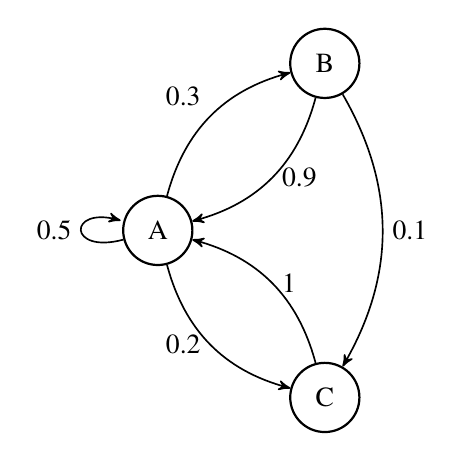
\begin{tikzpicture}[->, >=stealth', auto, semithick, node distance=3cm]
\tikzstyle{every state}=[fill=white,draw=black,thick,text=black,scale=1]
\node[state]    (A)                     {A};
\node[state]    (B)[above right of=A]   {B};
\node[state]    (C)[below right of=A]   {C};
\path
(A) edge[loop left]     node{0.5}         (A)
    edge[bend left]     node{0.3}     (B)
    edge[bend right, left]     node{0.2}      (C)
(B) edge[bend left,right]    node{0.9}      (A)
    edge[bend left,right]    node{0.1}      (C)
(C) edge[bend right, right]    node{1}      (A);
\end{tikzpicture}

The probability matrix belonging to this process looks like the following:

\[
\begin{matrix}
		& A		& B		& C \\
	A	& 0.5	& 0.3	& 0.2 \\
	B	& 0.9	& 0		& 0.1 \\
	C	& 1		& 0		& 0 \\
\end{matrix}
\]

\end{center}

Adding the $A,B,C$ is optional, but I find it gives more overview. The first
cell reads, the probobality of going from a to a.

\subsubsection{Stochastic}
A matrix where every row sums to1 is called a \emph{stochastic matrix}. Every
transition matrix is a \emph{stochastic matrix}.

\subsection{Sample path}
A \emph{sample path} of a markov chain is a specific specific realistion of
that chain.

\[ X_0,X_1,X_2,\dots\]

The $X_i$ are random variables.

\subsection{Markov process}
A \emph{Markov process} is a stochastic process $X_0, X_1, X_2, \dots$ such 
that:

\[ P\{ X_{n+1} X_n, X_{n-1}, \dots\}=P\{X_{n+1}|X_n\}\]
for $n \ge 0$

\subsubsection{Remarks}
If states are numbers, then often state space is denoted by $I$, with 
typical elements $i,j,k$.

A markov process is sometimes called a markov chain. These concepts are
equal.

If $S$ is countably infinite, then the probability transition matrix
can be represented as an ``open ended'' stochastic matrix.
\[
	P =
\begin{pmatrix}
	p_{1,1}	& p_{2,1}	& p_{3,1} & \cdots\\
	p_{1,2}	& p_{2,2}	& p_{3,2}	& \cdots\\
	p_{1,3}	& p_{2,3}	& p_{3,3}	& \cdots\\
	\vdots	& \vdots	& \vdots		& \ddots \\
\end{pmatrix}
\]
With markov proceci it is extremly important to beclear about the
\emph{cardinality of the state space} (finite, discrete, continues) and
the \emph{nature of time} (discrete, continuous)

A \emph{dead state} or a \emph{dead end} is a state that does not have
any outgoing arcs. An \emph{absorbing  state} is a state that has precisely
one outgoing arc with probability 1 to itself.

\subsection{Chapman-Kolmogorov equations}

\[P^{(n)}_{ij} = \sum_{all\mbox{\ }k} P^{(n_1)}_{ik} P^{(n_2)}_{kj} \]

It is convenient to list the $n$-step transition probabilities in a matrix.
\[
	P^{(n)} =
\begin{pmatrix}
	p^{(n)}_{1,1}	& \cdots	& p^{(n)}_{n,3} 	& \\
	\vdots	& \ddots	& \vdots	& \\
	p^{(n)}_{1,n}	& \cdots	& p^{(n)}_{n,n}	& \\
\end{pmatrix}
\]

In particiular $P^{(1)} = P$.

\subsubsection{Lemma}
Suppose $k+l=n$ Where $k,l\ge1$. Then $P^{(k)} \cdot P^{(l)} = P^{(n)}$

(I think this was proven)

$P^{(n)} = P^n$, this was definitivley proven. Not sure why you would
prove removing brackets, but whatever.

\subsection{Classes}
No this aren't default private structures (its a c++ reference).

Classes make dealing with large markov chains easier by grouping nodes
together. \emph{Open classes} allow the process to escape the class once
it enters a \emph{closed class} it will remain there forever.
A class is \emph{Transient} if a process can never reenter it, a
state is recurrent if it can. A process is multichain if there are
multiple recurrent classes, if there is just one reccurent class
its uni-chain.

A critical transition is a transition between classes.

A closed class doesn't have to be recurrent if there are infinite cases.
Otherwise a closed class is always recurrent.
An openclass is always transient.

\subsection{Markov reward}
A \emph{Markov reward process} is a markov process with rewards on
transitions. these rewards are real valued.

Markov rewards processes are also known as \emph{markov reward chain} or
\emph{valued Markov chains}.

example

\[
	P =
\begin{pmatrix}
	0.2	& 0.8 & 0 	& \\
	0.3	& 0	& 0.7	& \\
	0	& 0 & 1	& \\
\end{pmatrix}
\]
With reward matrix:
\[
	R =
\begin{pmatrix}
	1	& 2 & 0 	& \\
	0	& 0	& 3	& \\
	0	& 0 & 0	& \\
\end{pmatrix}
\]

\subsubsection{Total reward}

Let $\omega$ be a realisation of a Markov process:

\[\omega = s_0, s_1, \dots\]

where $s_0$ is a start state.
The rewards that accumulate are $r_1, r_2, \dots$:

\[ s_0 \xrightarrow[\mbox{reward } r_1]{} s_1 \xrightarrow[\mbox{reward } r_2]{} s_2\]

\paragraph{Definition}

$r_k | (s_0=1) : $ reward at kth step, given $s_0 = i$.
$R|(s_0=i),$ the \emph{total reward} : $(r_1 + r_2 \dots)|s_0=i,$
$V(i),$ the \emph{value} of state i : $E[R|s_0=i]$.

\subsection{The bellman equation}

\[V(i)=\sum_{all\mbox{\ }j} p_{ij}[r_{ij} + V(j)]\]

This system of linear equations enables us to compute state values in two
ways, by using algebra or by using iteration. Iteration you just wait until
convergence within a specified range. For this course iteration is enough.

\subsubsection{Utility pump}
A utility pump is a MRP in which at least one recurrent state possesses a
non-zero reward.
\subsubsection{Discount factor}
A \emph{dicsount factor} is a real number $0 \le \gamma < 1$. it represents
the probability to survive from one state to the next.

\paragraph{remarks} The discount factor is constant. The discount factor
does not impose a fixed cuttoff bound. It is a probablistic concept.

\subsubsection{Discounted reward}
Suppose a discount factor $0 \le \gamma < 1$. Then

\[V(i)=\sum_{all\mbox{\ }j} p_{ij}[r_{ij} + \gamma V(j)]\]

for every state $i$.

\paragraph{definition} A \emph{valuation} is a vector

\[v=Def
\begin{pmatrix}
	v(1) \\
	\vdots \\
	v(n)
\end{pmatrix}
\in \mathbb{R}^n
\]

\paragraph{definition} The \emph{expected immediate reward} at state $i$ is
the by $P_{ij}$ - probabilities weighted averaga of the $r_{ij}$ rewards:

\[C(i)=Def\sum_{all \mbox{\ }j} p_{ij} r_{ij} \]

The (vertical) vector of expected immediate rewards is denoted by $C$.

\paragraph{definition} The \emph{Bellman operator}:

\[B_p : \mathbb{R}^n \to \mathbb{R}^n : v \mapsto C + \gamma Pv \]

\subsection{Fixed point}
The value vector, $v^*$, of a discounted reward Markov process is a fixed
point of the $B_p$ operator:

\[ B_p(v)=v\]

\[
	v_0 \to B_p(v_0) \to B_p B_p (v_0) \to \dots \to B^n_P v_0
	\to \dots \to v^*
\]

\subsection{Example Markov reward process}
Consider the following markov reard process. Suppose a discount factor
$\gamma = 0.5$.

\[ \left\{ \begin{matrix}
		s: & s(r=1, p=0.4) & ; & a(r=4, p=0.6), \\
		a: & s(r=3, p=0.3) & ; & a(r=8, p=0.7), \\
		b: & s(r=2, p=0.5) & ; & b(r=5, p=0.5). \\
	\end{matrix}
\right. \]

\subsubsection{Transition diagram}
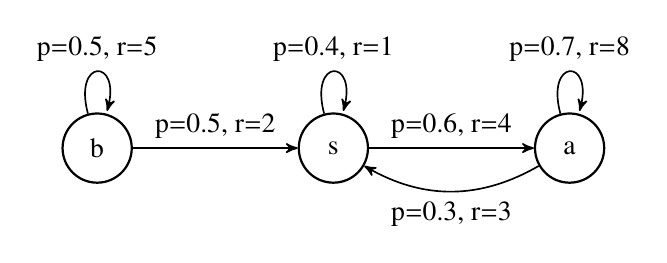
\begin{tikzpicture}[->, >=stealth', auto, semithick, node distance=3cm]
\tikzstyle{every state}=[fill=white,draw=black,thick,text=black,scale=1]
\node[state]    (S)                     {s};
\node[state]    (A)[right of=S]   {a};
\node[state]    (B)[left of=S]   {b};
\path
(S) edge[loop above]     	node{p=0.4, r=1}(S)
    edge[above]     		node{p=0.6, r=4}(A)
(A) edge[bend left,below]   node{p=0.3, r=3}(S)
	edge[loop above]     	node{p=0.7, r=8}(A)
(B) edge[above]    			node{p=0.5, r=2}(S)
	edge[loop above]     	node{p=0.5, r=5}(B);
\end{tikzpicture}
\subsubsection{Matrici}
\paragraph{Probability transition matrix}
\[
	P =
\begin{pmatrix}
	0.4	& 0.6 & 0 	& \\
	0.3	& 0.7 & 0	& \\
	0.5	& 0 & 0.5	& \\
\end{pmatrix}
\]
\paragraph{Immediate reward matrix}
\[
	R =
\begin{pmatrix}
	1	& 4 & 0 	& \\
	3	& 8	& 3	& \\
	2	& 0 & 5	& \\
\end{pmatrix}
\]
\subsubsection{Value evalutaion}
apply:
\[V(i)=\sum_{all\mbox{\ }j} p_{ij}[r_{ij} + V(j)]\]

\[ \left\{ \begin{matrix}
		V(s) = 0.4(1+\gamma V(s)) + 0.6(4+\gamma V(a)), \\
		V(a) = 0.3(3+\gamma V(s)) + 0.7(8+\gamma V(a)), \\
		V(b) = 0.5(2+\gamma V(s)) + 0.5(5+\gamma V(b)).
	\end{matrix}
\right. \]

With abusing notation:

\[ \left\{ \begin{matrix}
		s = 0.4(1+\gamma s) + 0.6(4+\gamma a), \\
		a = 0.3(3+\gamma s) + 0.7(8+\gamma a), \\
		b = 0.5(2+\gamma s) + 0.5(5+\gamma b).
	\end{matrix}
\right. \]

Just fill in the values recursevily to perform value iteration.

\subsection{Decision processes}
I'm gonna cover this subject poorly because its dead simple coming from an
IT background.

\begin{tabular}{ll}
	word & definition \\ \toprule
	decision tree & a simple directed tree stucture \\
	states & represented by verticies.\\
	Immediate rewards & represented by numbers along the edges. \\
	Decision alternatives & the outgoing edges, also called possible actions. \\
	Decision point & A state where a decision can be made. \\
	Finite decision tree & \brcell{A tree with a finite number of states, \\
		{\footnotesize Makes you wonder if there could be infinite number 
		of decisions in such a tree.}} \\
\end{tabular}
\\
The set of possible actions at state $i \in I$ is denoted by $A_i$.
The immediate reward for action $j$ at $i$ is denoted by $r_{ij}$.


\subsubsection{Policy}
A \emph{policy} specifies for every decision point $s$ a probability
distribution over $A_s$. A policy is typically denoted by $\pi, \tau\dots$.
If at $s$ the probability distribution puts all weight on one choice, the
policy is said to be \emph{pure} at $s$. Otherwise the policy is said to
be \emph{mixed} at $s$.

A \emph{run} of a policy is the \emph{actual execution} of that policy.
An \emph{realisation}, or \emph{sample path} of a policy is the trace of
that run.

The \emph{payoff} or \emph{total reward} of a run is the total sum of rewards
acuumulated in its realisation.

\subsubsection{Value function}
A \emph{value function} is any function $V: S \to \mathbb{R}$. The
\emph{expected payoff of a policy $\pi$}, given a certain starting state $s$:
	\[E[\pi|s_0=s]\]
	is called the value of $s$ under $\pi$, and is denoted by $V^\pi(s)$.
Value functions are compared in the following way:

\[ V_1 \le V_2 \Leftrightarrow_{Def} V_1(s) \le V_2(s), \mbox{for all states } s.\]

Policy $\pi$ is \emph{as good as} policy $\tau$ if $V^\tau \le V^\pi$. A policy
is \emph{optimal} if it is as good as any other policy. A value function is
\emph{optimal} if it is induced by a policy, and is as large as any other
such value function.

\subsubsection{Policy = strategy}
% this is the first what came to mind when I saw the policies.
In game theory, a policy is called a \emph{strategy} and a pure strategy is
sometimes called \emph{stationary} or \emph{deterministic}. A mixed strategy
is sometimes called \emph{probabilistic, non-stationary,} or
\emph{non-deterministic}.
% Imaginative with their non-*

An example of a pure policy is
\[ \tau = \{(r,b),(a,d),(b,e),(d,h),(f,i)\} \]

All the decisions are made, even if you already cut them off.
So you say (Start, End) for each node with choice.

Mixed policy:
\[ \tau = \{(r,\{(a, 0.2), (b,0.8)\}),(a,d),(b,\{(e, 0.7), (f,0.3)\}),
(d,h),(f,i)\} \]
% yes some really poor langauge design over here.

\subsubsection{Expected payoff}
$\pi$'s expected payoff, $E[\pi|s_0=r]$, can be computed recursivly with the
law of total expectation.

\subsubsection{Backward induction}
A decision between alternatives that leads to certain outcomes, is a certainty
itself.

Backward induction is applicable in \emph{directed acyclic graphs}(DAGs).

\subsubsection{Decision problem}
A \emph{decision problem} amounts to determining the set $\Pi^*$, where:

\[ \Pi = argmax_{\pi \in \Pi}(payoff(\pi))\]

Where $\Pi$ is the set of all policies.

For finite decision trees: Supppose at least one optimal policy exists.
If this policy is mixed, it may be replaced by an optimal pure policy,
such that, at every state, the payoff of the pure policy equals the expected
payoff of the mixed policy.

\subsubsection{Problems}
\paragraph{infinite width} no best policy, because you're valuating forever.
\paragraph{infinite depth} How to compare infinite total rewards (can't).
\paragraph{discount factor} The right decision is very dependent on the
discount factor. Counter intiuitive choices might be better for example.

\paragraph{Utility pumps}
If there is no discount factor policy is irrelivant (the reward will be
infinite no matter what you do). A tool is needed to kill infinity.
For example a finiti horizon, discount factor, or long-run average
payoffs.

In this course we will just use discount factors.

\paragraph{Investment} 
At cycle $a$, it is possible to `pump' 1 utitlity per iteration for as
long as a run lasts. At cycle $b$ it is possbile to `pump' $2$ utilities
per iteration.
In the long term it is better to be at $b$, but starting from $a$ this
requires an investment of $K$ rewardless transitions to get there.

\begin{center}
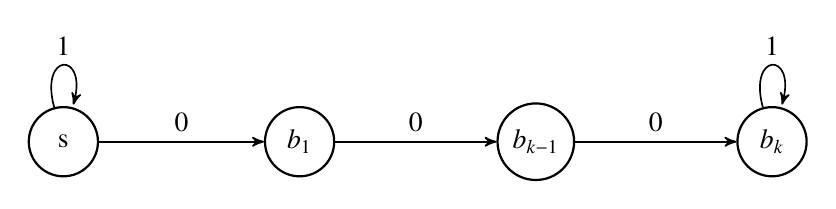
\begin{tikzpicture}[->, >=stealth', auto, semithick, node distance=3cm]
\tikzstyle{every state}=[fill=white,draw=black,thick,text=black,scale=1]
\node[state]    (S)                     {s};
\node[state]    (A)[right of=S]   {$b_1$};
\node[state]    (B)[right of=A]   {$b_{k-1}$};
\node[state]    (C)[right of=B]   {$b_k$};
\path
(S) edge[loop above]     	node{1}(S)
    edge[above]     		node{0}(A)
(A)    edge[above]    node{0}(B)
(B)    edge[above]     		node{0}(C)
(C)    edge[loop above]		node{1}(C);
\end{tikzpicture}
\end{center}

If $K \ne 0$ it is best to stay left if $\gamma < 2^{-1/k}$. (for the
proof see the slides, its to much math to copy in here).

\subsection{Policy improvement}

Recall the bellman equations for a Markov reward process:

\[ v = C+\gamma P v\]

To emphasise that $v$ depends on a probability transition matrix $P$:

\[ v^P = C^P + \gamma P v^P\]

In a \emph{decision problem}, $P$ is not chosen by nature, but by a 
\emph{decision maker}. In that case, $P$ is called a \emph{ixed Markov
policy}. and is denoted by $\pi$:

\[ v^\pi = C^\pi + \gamma P^\pi v^\pi\]

Each policy $\pi$ gives a value function $v^\pi$. THe objective is to find a
policy $\pi$ that maximises the value function $v^\pi$.

\subsubsection{First sketch}
A first sketch of a policy iteration algorithm:
\begin{enumerate}
	\item Start with an arbitrary policy $\pi$
	\item Compute $V_\pi$. (know as \emph{policy evaluation}).
	\item Improve $\pi$ locally to $\tau$.
	\item If $\tau \ne \pi$, then $\pi := \tau$, and go to 2.
	\item $\pi$ is optimal.
\end{enumerate}

\paragraph{Problem} Therer are to many ways to improve a policy.
For example if a state $s$ enables two actions, then any
mixed policy $(p, 1-p)$ may be tried locally. This gives
uncountably many (i.e., $|\mathbb{R}|$) alternatives!

Fortunally for discounted decision problems, locl search can be
restricted to pure policies only.

Let $\pi$ be apossibly mixed policy. For each state choose a decision
that is locally maximal:

% I'm not sure where the J is supposed to go.
\[M(i) \in argmax\{r_{ij} + \gamma V_\pi(j)\} \]

Define the pure policy:

\[ \tau_{ij} =_{Def} \delta_{M(i),j} \]

Then $\tau$ is a global improvement of $\pi$.

\subsubsection{Partial correctness}

Correctness  partial correctness + termination.

Partial correctness means: correct if the algrotihm terminates.
\emph{Policy iteration is partially correct:} any strict
local improvement induces a global improvment.
\emph{Policy iteration terminates:} each time a policy is improved,
the new policy is strictly better than the previous.

\subsection{Bellman optimallity}

If $\pi$ is optimal, it follows from the policy improvement thearom that

\[ V^\pi(i) = \underset{all\mbox{\ }j}{max}[r_{ij} + \gamma V^\pi(j)] \]

Removing explicit reference to the optimal policy automatically (more elegant).

\subsubsection{operator}
%seriously what is meant with operator?

% I'm assuming he means with exact the algebraic method and
% the aproximation is the itteration method.
For both methods (the exact as well as the approximation method),
a compacter notation is needed.

\[B: \mathbb{R}^n \to \mathbb{R}^n : v \mapsto
	\underset{all\mbox{\ }j}{max}[C_j + \gamma V(j)] \]

Where $C_j$ is the vector of rewards that emanate from state $i$.
Antoher way to write $B:$
\[\underset{all\mbox{\ }j}{max}[r_{ij} + \gamma V(j)] \]

$B$ does not depend on a policy or transition matrix. ($B_p$ does.)

\subsubsection{Fixed point}
The value-vector, $v^*$, of a decision problem is a fixed point of the
$B$-operator:
\[ B(v) = v\]


\subsection{Exam}
 For a given decision problem with a certain
discount factor.A pure policy sufices.
Do policy iteration, (a single iteration), do value iteration
(single iteration).

% That's all she wrote.

\end{document}
